% Chapter Template

\chapter{Fundamentals}\label{Chapter2} % Change X to a consecutive number; for referencing this chapter elsewhere, use \ref{ChapterX}

%----------------------------------------------------------------------------
%	SECTION 1
%----------------------------------------------------------------------------
It is impossible to exaggerate how vital meshing is in scientific computing and computer graphics. Meshes are the essential building blocks for visualizations, simulations, and numerous computations in these domains. As a discrete representation of a continuous domain, a mesh primarily consists of an interconnected network of vertices, edges, and faces (\cite{Zhang_2012}). The difficulty of creating meshes that correctly adhere to complicated and irregular geometry persists despite the advent of several meshing methods, and it is especially true when working with data-driven representations like Hermite data, where traditional approaches often fail to preserve topological consistency and geometric precision (\cite{Schaefer_2007}).
Because it provides the framework for several computational tasks, meshing is essential. Meshes in computer graphics allow for the development of 3D models and lifelike visualizations (\cite{Hristov_2022}). They provide numerical analysis, finite element analysis, and simulations of physical processes in scientific computing. The mesh quality directly influences the precision and effectiveness of these procedures. Researchers and engineers are constantly investigating novel techniques and algorithms to address the difficulties associated with mesh generation. They work to increase the fidelity of mesh representations, particularly in situations where geometric complexity and data-driven requirements demand precision and robustness. The continual search for cutting-edge meshing solutions emphasizes its critical importance in these fields (\cite{Hristov_2022}).

\section{Glossary} \label{Section 2.1}
This section briefly references the technical terms used in this work. The explanations are contextualized in the field of polygonization of isosurfaces. The only purpose of this section is to clarify terminology used throughout the thesis, not to generalize concepts.

\begin{itemize}
    \item \textbf{Cell:} A unit of volume in a 3D grid. In the context of isosurface extraction, a cell is often a hexahedron, but it could also be other shapes like a tetrahedron.
    \vspace{1.5mm}
    \item \textbf{Voxel:} A volume element representing a value on a regular grid in three-dimensional space. This is the 3D equivalent of a pixel.
    \vspace{1.5mm}
    \item \textbf{Cut Point:} A point where the isosurface intersects an edge of a grid cell.
    \vspace{1.5mm}
    \item \textbf{Grid:} A regular division of a 3D space into smaller, discrete units, often hexahedron or other polyhedra.
    \vspace{1.5mm}
    \item \textbf{Cartesian Grid:} This is a common type of grid, where the space is divided into cubes of equal size. The grid lines are parallel to the coordinate axes.
    \vspace{1.5mm}
    \item \textbf{Structured Grid:} As illustrated in Fig. \ref{fig:Regular-grid}, Structured grids are those in which the grid points can be ordered in a regular Cartesian structure, i.e., the points can be given indices (i, j) such that the nearest neighbors of the (i, j) point are identified by the indices (i±1,j±1) (\cite{David_2003}).
    \vspace{1.5mm}

    \begin{figure}
    \centering
    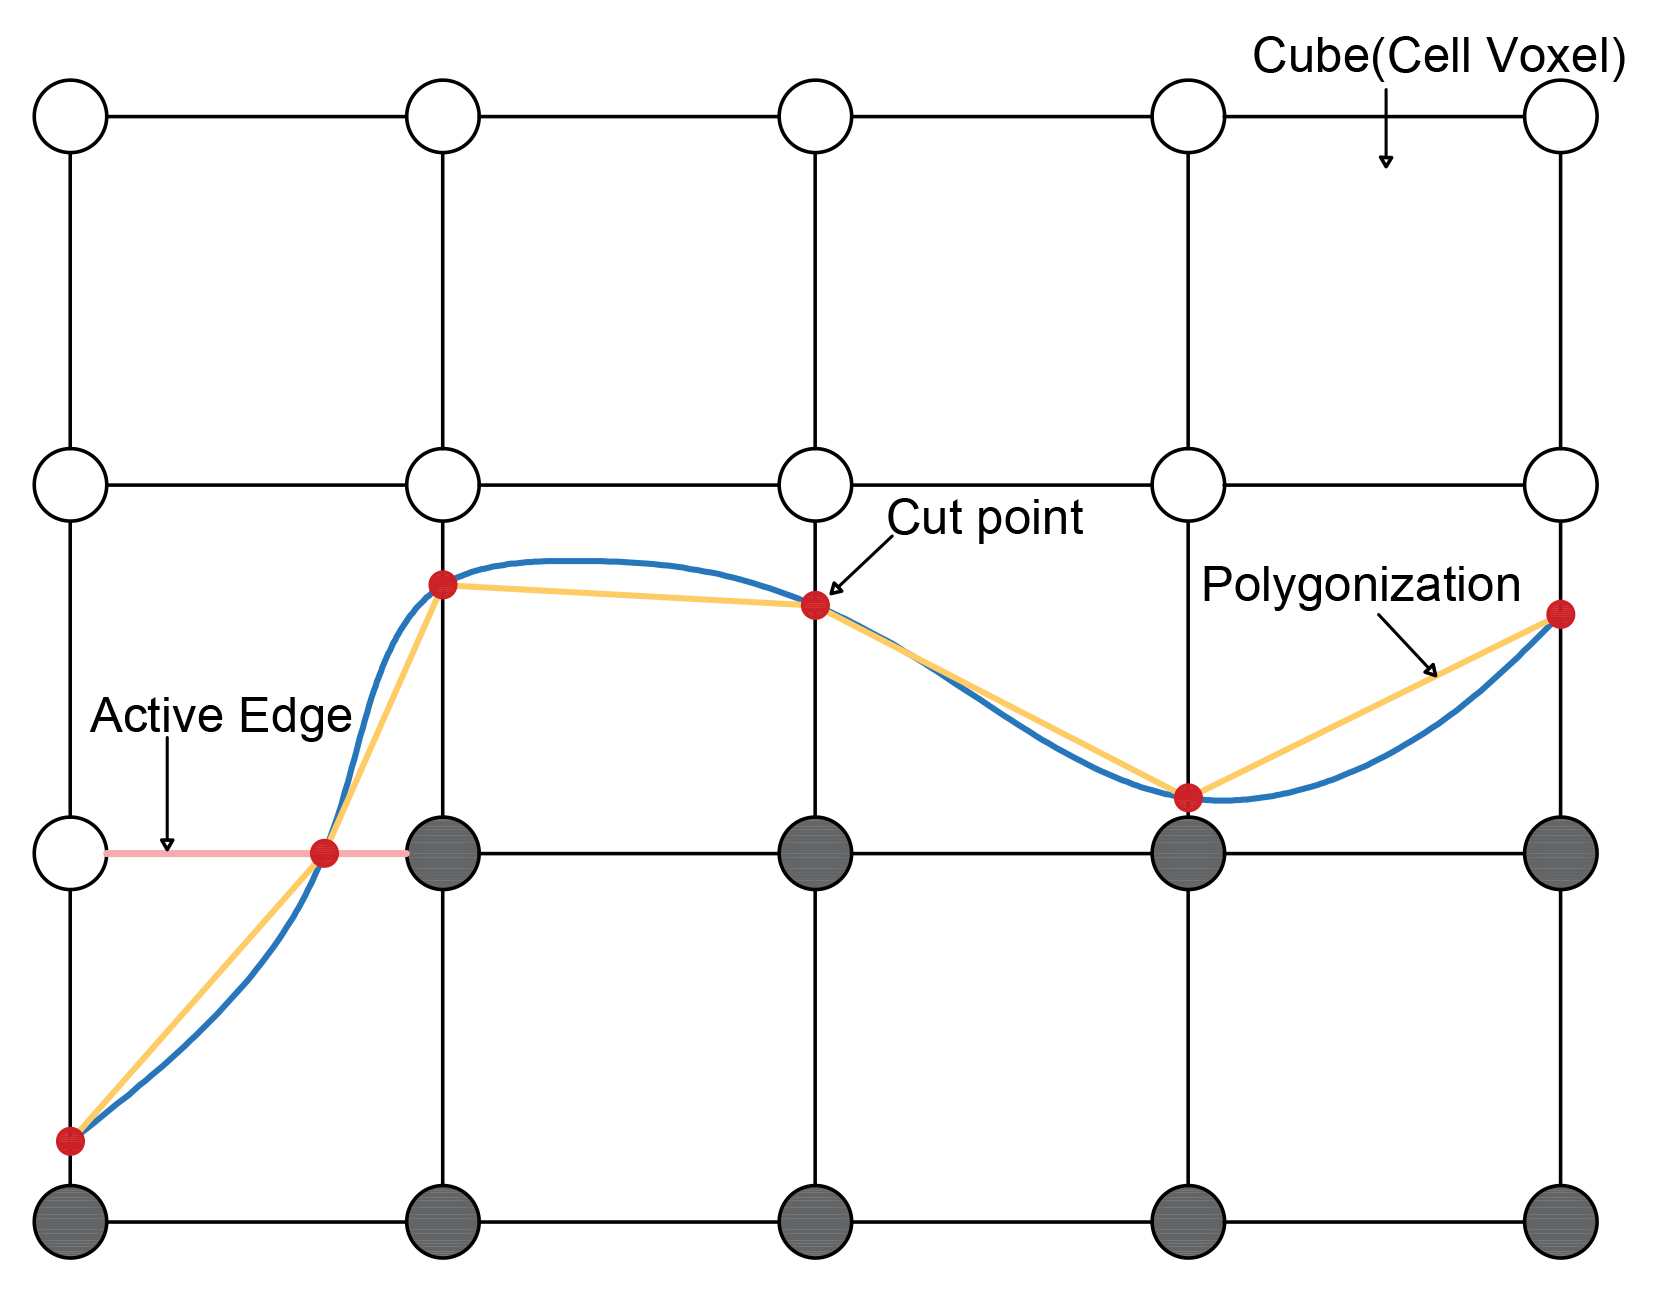
\includegraphics[height=0.5\textwidth,width=0.6\textwidth]{Figures/Regular_grid.jpg}
    \decoRule
    \caption{Regular grid}
    \label{fig:Regular-grid}
    \end{figure}
    
    \item \textbf{Unstructured Grid:} This is a grid where the cells can have arbitrary shapes and sizes. This grid type is often used for complex geometries or when the data is irregularly sampled.
    \vspace{1.5mm}

    \item \textbf{Adaptive Grid:} This is a grid where the cell size can vary across the space. This grid type is often used to represent spaces where the data has varying levels of detail or complexity. Octrees and quadtrees are types of adaptive grids. Fig. \ref{fig:quadtree} illustrates a quadtree, a tree data structure in which each internal node has exactly four children. An octree is the three-dimensional version of this structure, where each internal node has eight children, one for each octant of the 3D space.

    \begin{figure}
    \centering
    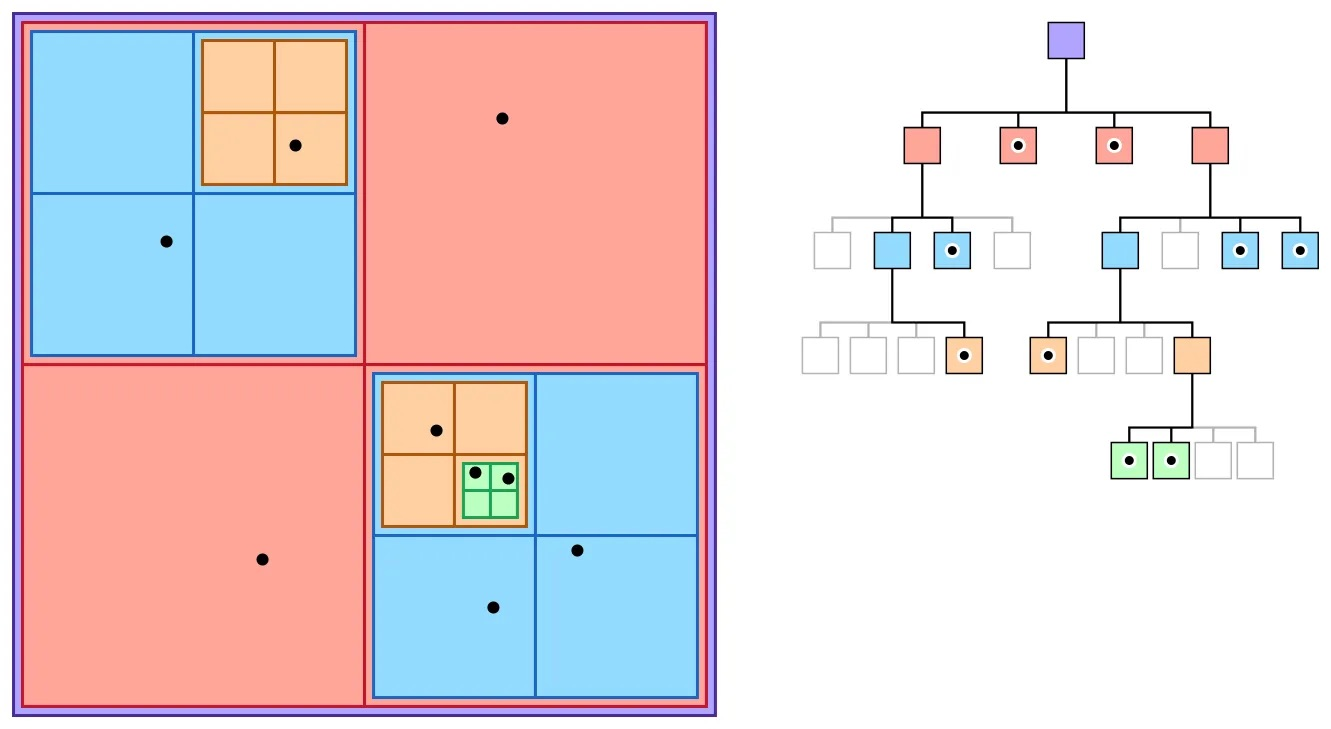
\includegraphics[height=0.45\textwidth,width=0.87\textwidth]{Figures/quadtree.jpeg}
    \decoRule
    \caption{Representation of quadtree}(\cite{image_quadtree})
    \label{fig:quadtree}
    \end{figure}
    
    \vspace{1.5mm}
    \item \textbf{Irregular Grid:} This is a grid where the cells can have different shapes and sizes. An unstructured grid is a type of irregular grid.
    \vspace{1.5mm}
    \item \textbf{Active Edge:} An edge of a grid cell intersected by the isosurface. The isosurface passes through the active edges of the grid.
    \vspace{1.5mm}
    \item \textbf{Isosurface:} An isosurface is a three-dimensional surface representing points of a constant value (or isovalue) within a volume of space. This volume of space is often represented as a 3D scalar field, which is a function that assigns a scalar value like density, temperature, and pressure to every point in a 3D space.
    \vspace{1.5mm}
    \item \textbf{Isovalue:} The isovalue is the specific value used to extract the isosurface from the 3D scalar field. For example, an isosurface might be extracted from a 3D Computed Tomography (CT) scan or Magnetic Resonance Imaging (MRI) at an isovalue representing bone density in medical imaging. This would result in a 3D surface representing the bones' or internal organ's boundary within the body. Figure \ref{fig:isovalue} shows the cross-section of a smooth sphere and its isosurface, marked with red, at two different isovalues, namely 50 and 200.
    
    % \begin{figure}
    % \centering
    % \includegraphics[width=\textwidth]{Figures/isovalue.png}
    % \decoRule
    % \caption{TO BE DELETED Multiple quad-trees (2D octrees) as \textbf{a} unstructured and \textbf{b} structured topologies}(\cite{image_quadtree_structured_unstructured})
    % \label{fig:types-of-grid-deleted}
    % \end{figure}

    \begin{figure}
    \centering
    \includegraphics[width=1.0\textwidth]{Figures/isovalue.jpg}
    \decoRule
    \caption{Cross-section of a smooth sphere (left), and surface marked with red iso-value set to 50 (middle) and iso-value set to 200 (right)}(\cite{image_quadtree_structured_unstructured})
    \label{fig:isovalue}
    \end{figure}
    
    \vspace{1.5mm}
    \item \textbf{Polygonization of isosurfaces:} The process of approximating isosurfaces using polygons, typically triangles, to create a mesh representing the surface in a 3D scalar field.
\end{itemize}


\section{Hermite Data} \label{Section 2.2}
Compared to scalar fields alone, Hermite data is a complex data format that provides a greater understanding of the underlying geometry. It encompasses derivatives at discrete places in space and scalar values (\cite{Hammarstrom_2013}). Hermite data offers a more thorough representation of geometric properties, including curvature, gradients, and shape changes, by including directional information through derivatives. In scientific and technical fields, this enhanced representation has proven essential for capturing complex structures and enabling more precise assessments (\cite{Markiewicz_Koperwas_2021}).

\paragraph{Challenges in Meshing Hermite Data:}
\begin{itemize}
    \item \textbf{Non-Uniform Data Distribution:} A non-uniform distribution of sample points within the spatial domain is a common feature of Hermite data. Variations in the local feature density or sample preferences cause this non-uniformity (\cite{Hammarstrom_2013}).
    \item \textbf{Varying Levels of Smoothness:} Derivatives of Hermite data reveal details on regional differences in smoothness. While some data areas may be smooth, others may have sudden shifts or discontinuities (\cite{Dai_2007}).
    \item \textbf{Discontinuities and Sharp Features:} Sharp edges, corners, and other geometric discontinuities can be represented via Hermite data. However, certain methods are needed to capture these properties correctly in a mesh (\cite{Hammarstrom_2013}).
    \item \textbf{Local Adaptation to Hermite Data:} The geometric diversity of Hermite data necessitates meshing methods that can dynamically adjust to changes in curvature and form. The tiny features and subtle fluctuations found in the data may be difficult to capture using conventional techniques that are not designed for Hermite data (\cite{Dai_2007}).
\end{itemize}

\section{Conformal Meshing and Geometric Accuracy} \label{Section 2.3}
Within computer graphics and scientific visualization, conformal meshing is seen as a crucial tenet, a passageway for depicting complicated real-world objects and data into coherent visual representations that may also be useful from an analytical standpoint. The fundamental skill of conformal meshing is the smooth transformation of complex geometric properties, such as curvature, sharp edges, corners, and other delicate subtleties, from the abstract world of data into concrete, detectable structures (\cite{Benkler_2008}). This process is the basis for accurate physical modeling, realistic visual simulations, and scientific comprehension across various fields. The core of conformality is the capacity to guarantee that the mesh, the discrete digital counterpart of the continuous physical environment, stays an accurate reflection of the underlying data. Contrary to traditional meshing techniques, which could unintentionally blur fine details or alter geometrical characteristics, conformal meshes accurately reflect the data's complexity. Viewers or analysts are given access to a more accurate picture of the actual item or phenomena when interacting with these meshes, offering insights that would not otherwise be possible (\cite{Dai_2007}).

The maintenance of geometric correctness is at the core of conformal meshing. Geometric correctness refers to how accurately the mesh represents the complex geometrical characteristics of underlying data, ensuring that critical details like forms, angles, and proportions are preserved in the meshed representation. This level of precision is especially crucial when working with complicated objects with various degrees of curvature or sharp features since any divergence from the original geometry might result in misleading representations or incorrect assessments (\cite{Benkler_2008}). Think about a scenario where fluid flow simulations are performed across the surface of an airplane wing. To accurately forecast aerodynamic behaviors, the complex curvature of the wing, including regions of high curvature near edges and corners, must be accurately represented. A solid modeling foundation built on a conformal mesh that correctly preserves these geometric details yields more precise insights into lift, drag, and other aerodynamic phenomena. Similarly, conformal meshing in medical imaging ensures anatomical features are correctly represented, enabling precise analysis for surgery planning or disease diagnosis (\cite{Chen_2022}). 
However, conformal meshing presents several difficulties in obtaining geometric precision. It necessitates overcoming the technical obstacles of discretization, interpolation, and error correction. The subtleties of data encoding, such as Hermite data, add smoothness variations and possibly discontinuities to the complexity (\cite{Chen_2022}). In order to address these nuances, meshing algorithms need to maintain topological consistency and integrity. Often, solving these problems requires striking a delicate balance between computational accuracy and efficiency. To achieve this balance, sophisticated algorithms and optimization techniques are used, guaranteeing that the resultant conformal meshes are accurate representations of the underlying data and suitable for simulations and real-time display. The quest for geometric correctness within conformal meshing is a dynamic and expanding frontier, necessitating interdisciplinary collaboration and novel strategies as the demands for increasingly elaborate and accurate representations increase (\cite{Benkler_2008}).

\subsection{Challenges in Achieving Conformal Meshing}
A key component of computer graphics and scientific visualization, conformal meshing offers the potential to convert complex data into accurate and aesthetically pleasing representations. However, there are obstacles to overcome in order to achieve geometric precision in conformal meshing (\cite{Dai_2007}). 
\begin{itemize}
    \item \textbf{Dissecting Complexity:} In conformal meshing, complexity may refer to various things, including the fine geometric details of objects and the depth of data representation. Sharp edges, subtle changes in curvature, and complicated surface patterns are just a few examples of the many characteristics that real-world objects frequently display. To capture these details, a mesh must be carefully resolved to retain a degree of geometric precision that accurately depicts the object's original shape. The difficulty comes from balancing the many smoothness levels, probable discontinuities, and uneven data distribution in Hermite data. Therefore, conformal meshing for Hermite data requires methods to deal with these difficulties while maintaining geometric precision and topological consistency (\cite{Chen_2022}).
    \item \textbf{The Efficiency Conundrum:} While pursuing geometric correctness is crucial, computing efficiency cannot be sacrificed, especially when real-time interactions or extensive simulations are required. The generation and rendering of high-resolution conformal models, which faithfully represent subtle geometric features, can be computationally taxing. Therefore, the difficulty is in effectively converting complicated data into meshes that balance complexity and processing expense (\cite{Alexa_2009}).
    \item \textbf{Strategies for Balancing Complexity and Efficiency:} Conscientiously employing techniques that use computational innovation and subject-matter expertise is necessary to balance complexity and efficiency in conformal meshing (\cite{Zhang_2012}). Utilizing adaptive mesh refinement, a method that dynamically modifies the mesh resolution based on the local properties of the data is one strategy. Because of this, regions with complex geometries can have better resolution, whereas smoother parts can use coarser components. Adaptive refinement maximizes geometric accuracy and computing economy by concentrating computational resources where they are most helpful. The effectiveness of conformal meshing can be improved by creating customized algorithms that use the built-in structure of the data (\cite{Markiewicz_Koperwas_2021}).
\end{itemize}



\section{Modeling Object Surfaces through Surface Extraction} \label{Section 2.4}
Surface extraction is a pivotal technique in computational geometry and computer graphics, bridging raw data representation and a structured geometric model. By extracting the surface from a set of data points or a volumetric representation, one can obtain a mesh or a set of primitives that closely approximates the original object's shape. This is particularly useful in applications like medical imaging, where accurate representation of organ surfaces can aid in diagnostics and surgical planning (\cite{Lorensen_1987}).

The process often involves techniques like the Marching Cubes (MC) algorithm, which is elaborated upon in Section \ref{Marching-Cubes}, that converts volumetric data into a triangulated mesh. This mesh can then be refined, smoothed, or further processed to achieve the desired level of detail and accuracy (\cite{Newman_2006}).

Once the surface is extracted, it serves as a foundational representation for various computational and graphical tasks. This structured geometric model enables more efficient computations, especially in rendering techniques like ray tracing. By accurately modeling an object's surface, we can achieve more realistic and precise visualizations, highlighting the critical role of surface extraction in the broader context of computer graphics and simulation (\cite{Whitted_1980}).

\section{Ray Tracing in Surface Extraction} \label{Section 2.5}
Ray tracing is an essential technique in computer graphics to mimic light behavior and, ideally, produce incredibly realistic visuals (\cite{Glassner_1989}). Finding the color and intensity of each pixel in the final picture requires tracking the movement of light beams as they interact with scene elements. This method accounts for the complex interactions between light and diverse surfaces, including reflection, refraction, and shadow casting (\cite{Parker_1999}).
Ray tracing excels in displaying isosurfaces in volumetric data, for example. Volumetric data, such as those from X-rays or scientific simulations, are three-dimensional data that define a volume's characteristics. The surfaces inside a volume with a constant value, such as a specific density or temperature, are known as isosurfaces (\cite{Aaron_2007}).

Ray tracing makes it possible to faithfully portray the intricate light interactions in volumetric data, producing very realistic and eye-catching renderings of isosurfaces (\cite{Glassner_1989}). The realism and depth of the produced pictures are improved by the accuracy of ray tracing in capturing minute fluctuations in lighting and shading. This skill is priceless in areas such as medical imaging, scientific visualization, and computer-aided design, where precise surface extraction and volumetric data visualization are essential for analysis and comprehension (\cite{Parker_1999}).

\subsection{Basics of Ray Tracing} 
The ray-tracing algorithm builds an image by extending rays into a scene and bouncing them off surfaces and toward sources of light to approximate the color value of pixels.
The computer graphics method of ray tracing models the behavior of light in a virtual scene. It starts by casting light onto the scene from the spectator's viewpoint (\cite{Haines_Akenine_2019}). As they go around the virtual world, these rays interact with the surfaces they come across. They replicate several optical effects dependent on the characteristics of those surfaces when they encounter objects, including reflection, refraction, and shadowing. The essential idea behind ray tracing is to identify the color of each pixel in a picture by examining the light that comes from the direction that corresponds to that pixel and hits the viewer's eye. This procedure entails following each ray's passage from the viewer's eye into the picture backward and analyzing the interactions it encounters (\cite{Haines_Akenine_2019}). As illustrated in Fig. \ref{fig:ray_casting}, The ray-tracing algorithm builds an image by extending rays into a scene and bouncing them off surfaces and toward light sources to approximate the pixels' color value.

\begin{figure}
    \centering
    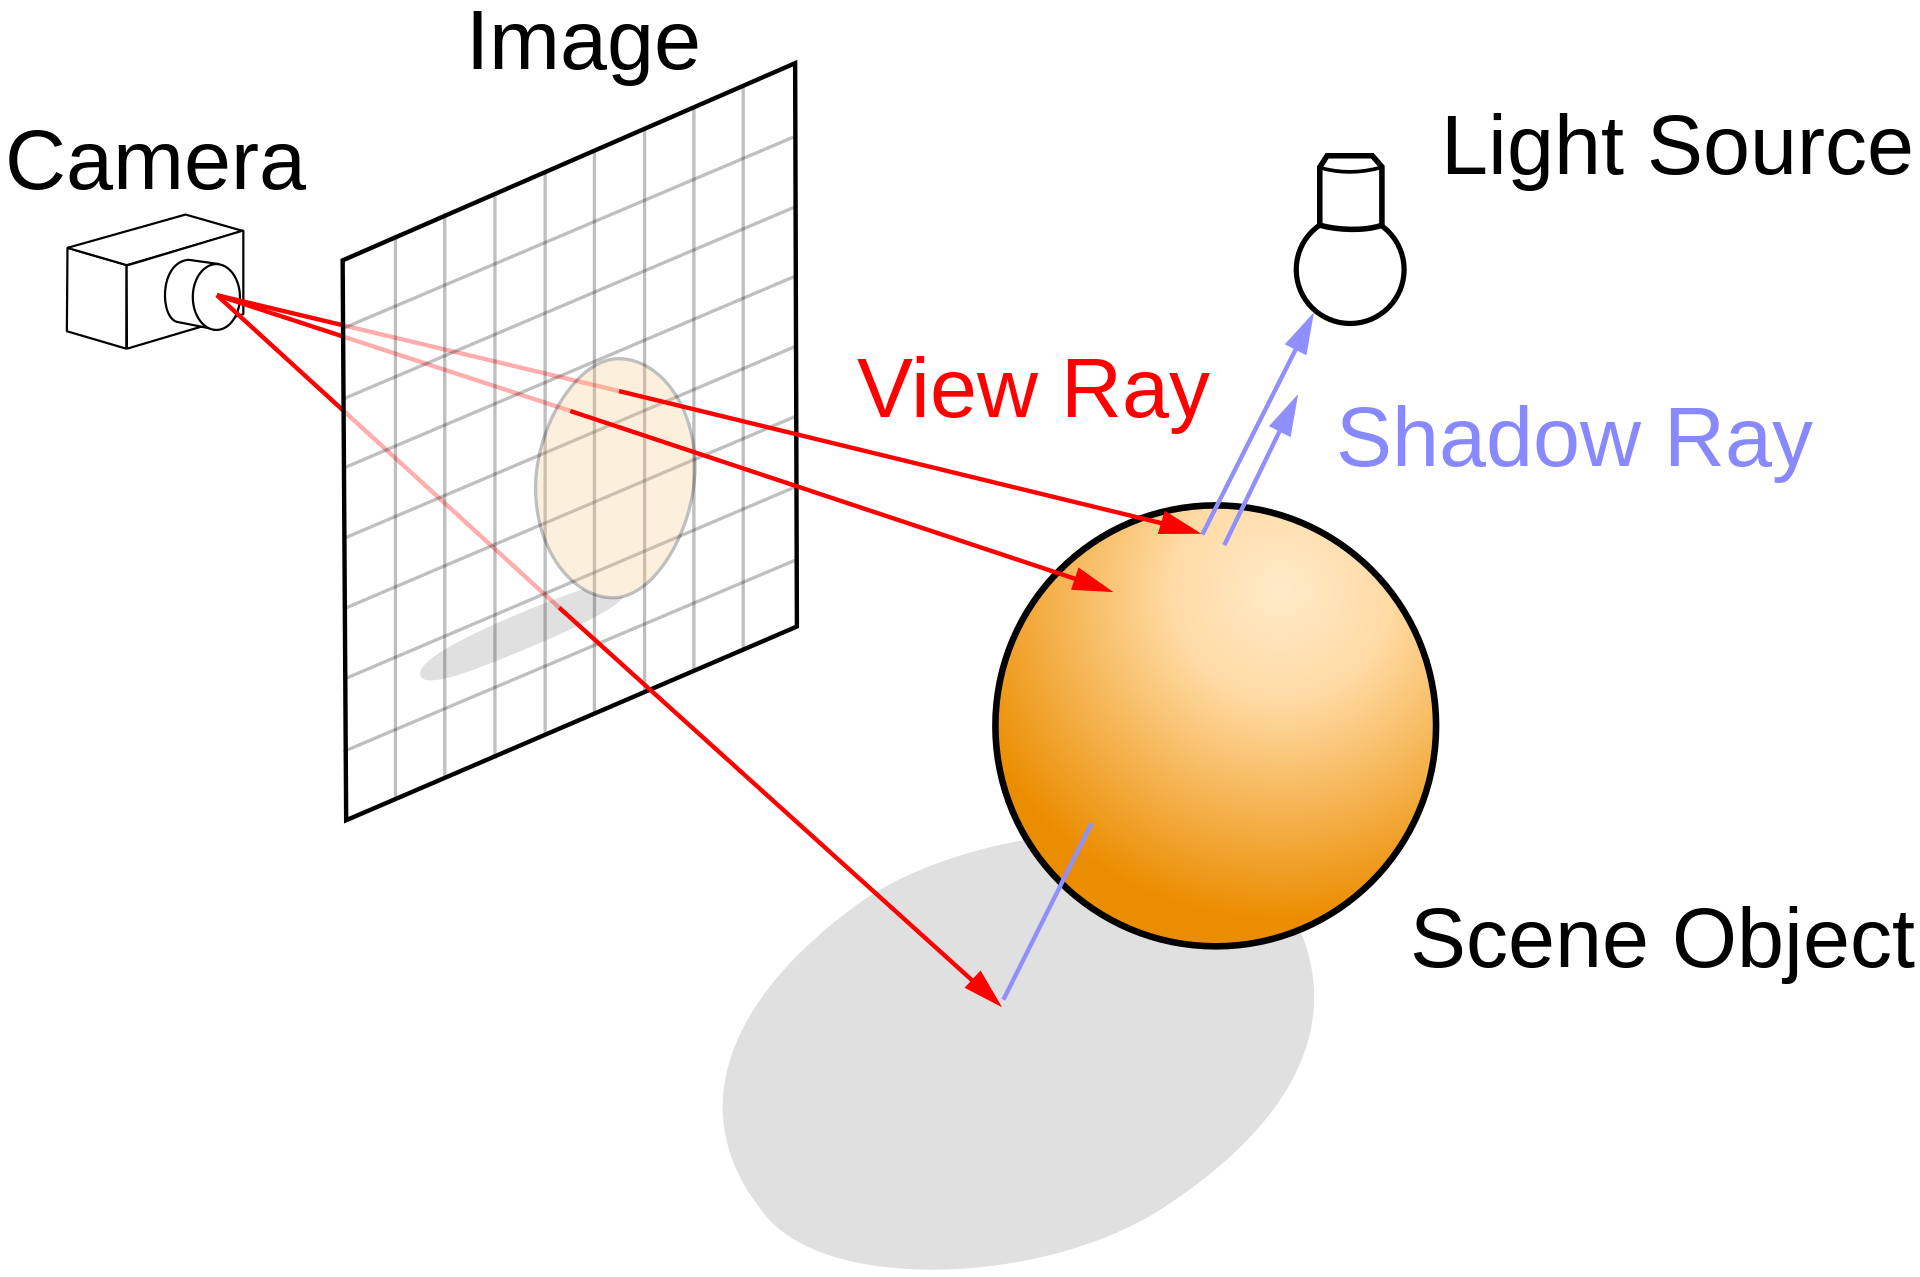
\includegraphics[height=0.4\textwidth,width=0.55\textwidth]{Figures/Ray_trace_diagram.png}
    \decoRule
    \caption{Ray tracing}(\cite{image_raytracingimage})
    \label{fig:ray_casting}
\end{figure}

Ray tracing permits the development of very realistic pictures by considering elements like the material qualities of surfaces, the angle of incidence, and the dispersion of light sources (\cite{Haines_Akenine_2019}). When objects partly obstruct light, they may capture subtle effects like soft shadows, which provide seamless transitions between lighted and shadowed parts. In order to replicate phenomena like depth of field, which causes objects to look in or out of focus depending on their proximity to the observer, ray tracing is also used. Additionally, it can mimic global illumination, considering indirect lighting and how light interacts with various surfaces in a scene and bounces off of them. Ray tracing has been a critical computer graphics technology since it was first used by \cite{Glassner_1989}, and it has continued to advance to produce generated pictures with higher degrees of photorealism (\cite{Haines_Akenine_2019}).

\subsection{Importance of Ray Tracing in Isosurface Extraction} 
Ray tracing, a cornerstone technique in computer graphics, is renowned for its ability to simulate intricate light interactions, producing highly realistic visuals. While it's often associated with rendering effects like shadows and transparency (\cite{Parker_1999}), the core functionality of ray tracing is pivotal for the specific application discussed in this work: surface point detection and the subsequent calculation of the Quadratic Error Function.

In the context of our research, ray tracing is employed not for its visual rendering capabilities but for its precision in detecting intersections. By firing a ray along each mesh line, we can accurately determine the point at which the ray intersects the surface. This intersection, or "hit point," along with the normal to that point, becomes instrumental in our calculations.

By accurately visualizing and analyzing complex structures and occurrences, integrating isosurface extraction with ray tracing helps researchers and scientists better interpret volumetric data. Precisely depiction of isosurfaces is crucial for efficient data processing and interpretation in various sectors, including engineering, scientific visualization, and medical imaging (\cite{Dai_2021}).

\subsection{Overview of Intel Embree API} \label{Intel-Embree-Overview}
Ray-tracing kernels with strength and speed are available via the Intel Embree API (\cite{Sato_2021}). It provides highly optimized methods for quickly computing ray-primitive crossings and is mainly created to use contemporary CPU architectures' capabilities. Embree is an excellent option for computationally demanding applications like isosurface extraction because the accuracy of ray tracing computations is essential. Embree may be easily integrated into various applications because of its modular design. Developers may use Embree's optimized ray tracing capabilities, assuring quick and precise calculations, by smoothly integrating Embree into their applications. The API offers adaptable and effective methods that let programmers use ray tracing on CPUs (\cite{Ingo_2014}).
Embree's capability to handle dynamic scenarios with ease is a noteworthy feature. As a result, Embree enables real-time interactions and dynamic visualizations in situations where the scene geometry varies over time. Embree is a popular option because of its capabilities for applications like interactive simulations, virtual reality, and gaming that need immediate response and fluid visualization. Developers may use Embree to create high-performance calculations and realistic visualizations using its optimized ray-tracing kernels. The API is an invaluable resource for various applications that need both speed and precision in ray tracing operations due to its emphasis on practical ray-primitive intersection computations, its modular design, and its support for dynamic scenes (\cite{Sato_2021}).

While the Intel Embree API is primarily designed for optimized ray tracing on CPUs, it is worth noting that the API also supports hardware-accelerated ray tracing on Intel GPUs through the SYCL programming language. This GPU support can significantly enhance the performance of ray tracing applications, especially when real-time graphics are a priority.

However, the CPU remains a more suitable choice for applications that do not demand real-time processing. Here are some reasons why the CPU version of the Intel Embree API is preferable:

\begin{itemize}
    \item \textbf{Maturity and Testing}: The CPU version of Embree is more mature and has undergone extensive testing, ensuring reliability and stability.
    \item \textbf{Wider Support}: It is more widely supported, allowing integration with a broader range of applications.
    \item \textbf{Ease of Use}: The CPU version is more straightforward to learn and implement. Unlike the GPU version, it does not necessitate expertise in GPU programming paradigms.
\end{itemize}

In summary, while the Intel Embree API offers enhanced performance on GPUs, its CPU-focused design is particularly advantageous for tasks, prioritizing accuracy, computational intensity, and ease of use over real-time responsiveness.

\section{Challenges in surface Extraction} \label{Section 2.6}
A strong method for analyzing and visualizing 3D scalar fields is surface extraction. However, the nature of the data, techniques, and expected results provide several difficulties.
\subsection{Data Resolution and Quality}
The resolution of a dataset dramatically influences the quality and detail of the extracted surface during isosurface extraction. Surfaces that are simplistic and devoid of finer features may be produced by low-resolution data when sample points are sparser. This might reduce the accuracy and realism of the extracted surface by causing the loss of crucial details and features in the visualization (\cite{Knoll_2021}).

On the other hand, high-resolution data captures a larger number of sample points, enabling a more accurate representation of the underlying scalar field (\cite{Knoll_2021}). Surfaces with minute features and slight data variances are produced as a consequence. High-resolution data processing, however, may be computationally costly. The growing amount of data points needs additional computing capacity and processing power to execute the required computations. Longer processing times may result, particularly in complicated or real-time systems where prompt feedback and interactive features are essential (\cite{Knoll_2021}).

Therefore, it is crucial to balance computing efficiency and resolution. It entails choosing a resolution that will capture the necessary degree of detail while considering the application's performance needs and the available computing resources. This compromise makes the extracted surface accurate and aesthetically pleasing without compromising performance or real-time responsiveness (\cite{Knoll_2021}).

\subsection{Noise and Artifacts}
Noise is a typical feature of real-world datasets, which may harm the precision and quality of the retrieved surface during isosurface extraction. Noise is the term for arbitrary or undesirable oscillations in the data that do not accurately represent the underlying scalar field's genuine characteristics. These variations may be caused by many things, including measurement blunders, sensor noise, or built-in constraints in data-collecting procedures (\cite{Savchenko_1995}).
To ensure the fidelity of the extracted surface, it is imperative to address these challenges. While there are techniques to mitigate noise, they might inadvertently suppress genuine data features. Similarly, rectifying artifacts without domain-specific knowledge can be challenging. The overarching challenge is to discern and address noise and artifacts without compromising the integrity of the actual data features.

\subsection{Computational Overhead}
Extracting surfaces from big datasets may be computationally taxing for real-time or interactive applications. The computational burden of surface extraction rises as datasets are more extensive and complicated. Optimized algorithms and effective data structures are required to minimize processing time and memory utilization to handle this. These methods seek to accelerate surface extraction, allowing quick calculations and responsive user interfaces even for complex and large datasets (\cite{Lewiner_2003}).

\subsection{Ambiguities in Scalar Fields}
During the surface extraction process in scalar fields, locations where the values vary quickly create a problem. One of the primary issues is the ambiguity that arises when determining the topology of the isosurface in regions where the scalar field values are close to the isovalue.

Several solutions have been proposed to address these ambiguities. \cite{Nielson_1991} introduced the "asymptotic decider" to resolve the ambiguity based on the local behavior of the scalar field.

Despite these advancements, ambiguities in scalar fields still need to be solved, requiring careful consideration to ensure accurate and topologically correct surface extraction.

\subsection{Hardware and Software Limitations}
The limits of the hardware and software platforms in use also impact how effective surface extraction is. Powerful hardware is often needed to handle modern datasets promptly. Software solutions must also be tailored to their particular hardware, using parallel processing strategies, GPU acceleration, and other cutting-edge computing approaches.

\section{Summary}
In this chapter, we delved deep into the intricacies of surface extraction, emphasizing its significance in various domains like computer graphics, scientific visualization, and medical imaging. We started by understanding the foundational role of meshes in representing continuous domains and the challenges posed by data-driven representations like Hermite data. The glossary section provided a comprehensive overview of the technical terms, ensuring clarity in the subsequent discussions.

We then explored the nuanced challenges posed by Hermite data in meshing, emphasizing the non-uniform distribution, varying levels of smoothness, and the presence of discontinuities. The discussion on conformal meshing highlighted the importance of geometric accuracy in representing real-world objects and the challenges in achieving it. The balance between computational accuracy and efficiency was underscored, emphasizing the need for innovative algorithms and optimization techniques.

The section on surface extraction provided insights into the process of converting volumetric data into structured geometric models, with ray tracing playing a pivotal role in achieving realistic visualizations. The challenges in surface extraction, ranging from data resolution to ambiguities in scalar fields, were discussed in detail, highlighting the complexities involved in the process.

This chapter provided a comprehensive overview of the complexities and nuances associated with meshing and surface extraction. As we move forward, these foundational concepts will serve as a backdrop for more in-depth discussions on specific algorithms and techniques in the realm of isosurface extraction.